\documentclass[10pt,a4paper]{article}
\usepackage[margin=0.88in]{geometry}
\usepackage[T1]{fontenc}
\usepackage[utf8]{inputenc}
\usepackage{lmodern,graphicx,booktabs,tabularx,array,amsmath,amssymb,xcolor,microtype,enumitem}
\usepackage[hidelinks]{hyperref}
\usepackage[font=small,labelfont=bf]{caption}
\setlength{\parindent}{0pt}
\setlength{\parskip}{5pt}
\renewcommand{\arraystretch}{1.16}
\newcommand{\hold}{\textsc{Unresolved}}
\newcommand{\reported}{\textsc{Author-reported}}
\newcommand{\raw}{\textsc{Raw-replayed}}
\newcommand{\papertype}{\textbf{Scientific development manuscript --- not the completed systematic review or a submission-ready copy.}}
\title{From Photovoltaic Imaging Scores to Source-Supported Claims\\
\large Dataset Ancestry, Physical Units and Model Selection: An Experiment-Indexed Evidence Audit}
\author{Anonymous research draft --- author metadata pending}
\date{8 November 2026 \;|\; Research-development version R57 (temporal and thesis source evidence; not final PRISMA)}
\begin{document}
\maketitle
\begin{center}\small\papertype\end{center}
\begin{abstract}
Performance claims for AI-assisted photovoltaic (PV) inspection depend on the experimental unit, source ancestry, checkpoint-selection rule and metric denominator. We present an experiment-indexed evidence audit with reproducible source-bound diagnostics rather than a pooled model leaderboard. Reanalysis of nine published cross-plant infrared tasks reconstructs 54 AUROC cells; the preferred classifier under target-label-selected checkpoints differs from both other-plant validation selections in three tasks. In original Sandia PV-IV-EL metadata, 616 acquisitions span 438 source module identifiers and 613 unique IV paths. Across 100 random row partitions, a mean 55.17 module identifiers cross training and test; source-module-grouped partitions enforce zero overlap. A frozen non-imaging Ridge model predicting measured-to-nameplate IV power ratio on 598 eligible rows yields mean MAE 0.8650 versus 0.8790 ratio percentage points for row-wise versus module-grouped tests, showing that source overlap does not automatically imply inflated scores. In a separately locked future-calendar test of 139 IV observations, 56 test module identifiers were previously observed. Removing 59 earlier training rows associated with test modules changes same-test Ridge MAE from 1.3691 to 1.6411 ratio points, but also changes training composition and does not isolate a causal overlap effect. Pinned public electroluminescence segmentation directories contain no identical train/test filenames yet 22, 33 and 34 shared parsed name-source families across three releases. A 2024 author thesis describes a CFVS source-module-number/cell-coordinate naming example, without verifying the original trained paper's exact physical-parent manifest. The analysis separates observable source support from untested image-model leakage or site-transfer claims. Full-text eligibility, independent human screening and PRISMA/PRISMA-S remain incomplete; this is a research-development audit, not a completed systematic review.
\end{abstract}
\noindent\textbf{Keywords:} photovoltaics; electroluminescence; infrared thermography; physical-unit independence; dataset ancestry; grouped validation; reproducibility; experiment-indexed evidence.

\section{The research question and originality boundary}
Photovoltaic inspection studies report classification accuracy, F1, AUROC, average precision, mAP and segmentation measures under different acquisition regimes. A thermogram of a module, a crop of one cell, multiple video frames of the same module, a synthetically augmented image, and a newly inspected PV plant are not interchangeable experimental units. A numerical performance figure is therefore evidence about a particular \emph{target, source population, partition and selection rule}; it is not itself a demonstration of external transfer.

Several existing reviews have already summarized PV faults, EL and infrared imaging, machine-learning models, datasets and general field-robustness limitations. Ali, Zafar and Kim provide a systematic imaging-focused review of 2021--2024 studies \cite{ali2026}; Meena and Gawre synthesize 95 AI fault-diagnosis studies across modalities \cite{meena2026}; an IEEE Access review discusses diagnostic techniques and AI datasets and evaluation metrics \cite{ieee2026}; and Rahman and Srivastava integrate detection, classification and localization across fault families \cite{rahman2026}. Pillai and colleagues' publisher-listed review, indexed for a 2027 volume, explicitly distinguishes fault-visibility benchmarking from naive metric comparison \cite{pillai2027}. These reviews are substantive prior work. Consequently, broad statements such as ``datasets are small,'' ``more external validation is needed,'' or ``methods cannot be directly compared'' are \emph{not} claimed as new contributions here.

Earlier structured comparative work directly overlaps the source-data themes: Li and coauthors already tabulated datasets, original/augmented images and some train--test partitions in a 2021 neural-network PV fault-diagnosis review \cite{li2021}. Nasri and coauthors compared multimodal datasets and fusion methods at study level \cite{nasri2026}; Wang and Xing reviewed nondestructive PV defect AI \cite{wangxing2026}; and Lu and coauthors proposed a qualitative multi-indicator comparison of fusion methods \cite{lu2026}. These are direct predecessor contributions, not merely generic warnings about external validation. Their full-text coverage of each evidence field is not yet exhaustively adjudicated, so methodological priority cannot be asserted from abstract silence.

Cross-validation of hierarchically or spatially structured records is a well-established methodological challenge \cite{roberts2017,varoquaux2018}. Leakage taxonomies and model information sheets also predate this work \cite{kapoor2023}. We therefore do not claim invention of grouped validation, leakage warnings or evidence cards. Our narrower test is whether an auditable hierarchy of source-file, candidate-parent and declared physical-parent identifiers changes a result's \emph{admissible interpretation}, and whether a separate fixed predictor actually shows a performance contrast.

The potential additional contribution is an auditable, \emph{result-specific} bridge from source evidence to admissible inference. We ask not only whether a paper describes AI on EL or IR, but which individual result was obtained under which versioned source, original physical acquisition, partition, checkpoint-selection rule and denominator. One report can therefore generate several different experiment/result records while retaining one bibliographic study identity. The proposed record is an audit instrument, not a composite methodological-quality index or a claim of priority over every preceding review. Whether this is a sufficiently distinct systematic-review contribution remains to be established against the complete full-text prior-art set.

\section{Evidence corpus and study-design status}
\subsection{Search provenance and selection status}
The frozen 31 October 2026 source archive contains 21 native Scopus, Web of Science and IEEE Xplore exports comprising 8,326 provider record rows. A conservative identity pass groups these into 5,440 \emph{provisional} bibliographic work identities, preserving unresolved DOI/title collisions, conference-to-journal relationships, corrections and multi-record aliases. The identity-group count is not yet a fully adjudicated deduplicated-study denominator. A previous priority frame of 599 identities was used to organize deeper source retrieval, not to define the full included population.

As of the independent 7 November R47 Batch27 source-and-custody readback, the two nonoverlapping AI-assisted source-screen workloads have completed 2,588/2,588 and 1,375/2,588 records, respectively (3,963 of 5,176 assigned \emph{screening records}). Those 5,176 assignments are worker source-screen workload rows, not 5,176 unique eligible clinical-style studies, and should not be substituted into a PRISMA flow. No completed full-text eligibility round, independent second-human screener, agreement statistic or final included-study count is claimed. PRISMA 2020 and the PRISMA-S search-reporting extension are planned reporting targets \cite{prisma,prismas}; the latter requires a reproducible database/platform/query/date record, beyond an assertion that a search was performed.

This version concentrates on a bounded reproducible science demonstration rather than extrapolating the partial screen to prevalence estimates. The executed illustrative source set is purposive. Three reports are matched to frozen identities and one original-publisher report, \c{C}al{\i}\c{s}an (2026), was discovered \emph{after the searches were frozen} despite its publisher publication date of 21 October 2026. It is a separately labeled contemporary source, \emph{not silently inserted} into the 31 October export frame. An exact DOI/title lookup against the archived 5,440-identity metadata register returned no match, which establishes that narrow register fact but does not establish why a record was absent from the original institutional query results.

\subsection{Experiment-indexed evidence record}
Each proposed record has a stable source-to-result path:
\begin{center}
\fbox{\parbox{0.92\linewidth}{\centering\small
\textbf{Report and version} $\longrightarrow$ \textbf{source release / annotation origin} $\longrightarrow$ \textbf{physical acquisition parent}\\[3pt]
$\longrightarrow$ \textbf{image / crop / augmentation descendants} $\longrightarrow$ \textbf{train--validation--test assignment}\\[3pt]
$\longrightarrow$ \textbf{model / checkpoint-selection exposure} $\longrightarrow$ \textbf{metric, denominator and bounded claim}
}}
\end{center}
A record separates \emph{reported} facts from \emph{replayed} facts. In particular, author statements of module-grouped sampling are meaningful evidence and are recorded positively; they are not rebranded as independent raw-manifest verification. Conversely, unreported image-parent mapping is an identifiability limit, \emph{not proof} of leakage or misrepresentation. The record retains a source URL, source tier, exact source section/table, and missing-value state for every stronger inference.

\begin{table}[ht]
\centering\small
\caption{Evidence tiers and defensible claims. Passing a lower-tier source check never automatically grants a stronger validation certificate.}
\begin{tabularx}{\linewidth}{@{}p{2.25cm}X X@{}}
\toprule Evidence tier & What it may establish & What it cannot alone establish \\
\midrule Provider or publisher abstract & Report identity, modality, indicative task, author-quoted headline outcome & Detailed split manifest, physical-parent independence, complete test denominator \\
Original Methods and tables & Author-described source population, split policy, checkpoint selection, task and metric values & Independent correctness of unprovided image-to-module ancestry \\
Owner code and versioned metadata & Release/commit identity and inspectable processing, when corresponding artifacts exist & Same experimental sample identity across papers without an explicit join \\
Raw image--parent replay & Literal zero cross-partition overlap for a defined mapped parent and version & Universal site transfer or absence of every possible nuisance/selection dependence \\
\bottomrule
\end{tabularx}
\end{table}

\subsection{A source-only, reproducible diagnostic}
To demonstrate why the checkpoint rule belongs in every result record, we re-tabulated Table~5 of Bommes et al. \cite{bommes2022}. Its nine source-to-target \emph{cross-plant} rows compare a contrastive k-nearest-neighbor method with a cross-entropy classifier. For each task and classifier the table reports three AUROC percentages: the model selected using validation plant 0, model selected using validation plant 1, and the \emph{Best} score selected on labeled target data. This yields $9\times2\times3=54$ printed metric cells. The authors explicitly distinguish the target-best choice from feasible selection on another labeled PV plant; their published design also reports module-level train/test grouping and cross-plant evaluation. We do not retrain their models or re-estimate confidence intervals from per-run data.

For source--target task $t$, classifier $m\in\{C,E\}$ and selection condition $s\in\{0,1,T\}$, let $U_{tms}$ be the \emph{printed} AUROC percentage. Define the within-condition method separation and a descriptive selection-condition difference as
\begin{align}
\Delta_{ts}&=U_{tCs}-U_{tEs},\\
G_{tms}&=U_{tmT}-U_{tms},\quad s\in\{0,1\}.
\end{align}
Here $T$ is the target-label-selected Best, not a blind test estimator. $G$ is \emph{not} an experimental causal effect or a corrected estimate of generalization; it compares different reported checkpoint choices. A strict reversal is counted only when the sign of $\Delta_{tT}$ differs from the signs of both $\Delta_{t0}$ and $\Delta_{t1}$. The printed two-decimal precision is retained. The supplied reproduction script reads the hash-pinned 54-cell extraction and checks the task count, sign flips and extrema.

\subsection{Executed public data and outcome-specific controls}
The Sandia PV-IV-EL catalog describes 613 paired measurement sets and 438 identified modules \cite{sandia2025}; the raw source \texttt{AnonDB.csv} read in this audit has SHA-256 \texttt{8fe45044...083440e}, 616 rows and 438 unique nonblank \texttt{Mod\_ID} values. The full 64-character hash is in the code package. No original row is removed to reconcile the catalog's 613-set headline. For the physical-unit membership diagnostic, fixed seeds 20261108--20261207 generated 100 disjoint 493/123 row partitions and 100 separate 493/123 whole-\texttt{Mod\_ID} partitions. The latter keeps all rows for one module on the same side. We check source-key intersections explicitly rather than assuming file count implies parent independence.

A separately locked, \emph{non-imaging} negative-control model evaluates the measured electrical ratio $y=P_{\rm mp,IV}/P_{\rm mp,nameplate}$, not an EL crack label or power loss inferred from a segmentation mask. Prespecified complete-covariate eligibility yields 598 rows/420 module IDs. A fixed Ridge ($\alpha=10$) model uses manufacturer/model, wafer type, nameplate rating, area, outdoor exposure and exposure step, but not \texttt{Mod\_ID}, IV-derived output/current/voltage, image pixels or target information. Across 100 row-versus-whole-module 478/120 splits, preprocessing is fitted on training data only. MAE is reported in percentage points of $y$ and the constant $\hat y=1$ is a reference. These split populations differ by design: errors cannot be interpreted as a randomized causal effect of overlapping parents. The original IV/EL imaging source supports a later separate pixel-based model \cite{byford2025}, but no pixel-based score was produced here.

A further original-source chronology sensitivity was specified before inspecting new predictions. Complete source-IV calendar days define a future holdout beginning 9 February 2021, with unchanged future test rows for two Ridge fits: all earlier metadata rows or only earlier rows whose source \texttt{Mod\_ID} does not occur in that future test. The latter deletion changes the size and composition of training, so the same-test score contrast is descriptive rather than causal. A prespecified 100-seed equal-size exclusion control retains earlier observations of future-seen modules, but remains composition-confounded. A metadata-only dual-EL-path and seven-day IV date check measures potential source support, not actual TIFF readability. These analyses retain the R52 predictor and continuous IV power-ratio endpoint, with no pixel input or model tuning.

A third diagnostic reads exact Git subtree names from three dated releases of the public Pratt et al. EL segmentation benchmark \cite{pratt2023}. We test exact filenames, augmentation-normalized crop names and only the strict candidate-family prefix before an \texttt{\_r\#\_c\#} crop suffix. That parsed family is \emph{not} asserted to be a physical module identifier. The release-to-published-model mapping and source image/mask bytes were not replayed. All three audits are purposively selected methodological controls, not a population estimate of review-study behavior.

\section{Source-linked methodological results}
\subsection{Checkpoint choice changes the descriptive ordering}
Figure~\ref{fig:selection} compares the two classifiers at each reported selection condition. It plots \emph{within the same source--target task} rather than aggregating accuracies across heterogeneous studies. The signed method separation reverses between target-best and both validation-plant selectors on B$\rightarrow$E, B$\rightarrow$F and F$\rightarrow$A: \textbf{three of the nine published cross-plant tasks}. This is an illustrative property of that study's printed results, not an estimate of how often such reversals occur in PV research. In B$\rightarrow$E the target-best difference is only $-0.02$ AUROC percentage points; its small magnitude is important when interpreting the apparent winner. The corresponding B$\rightarrow$F and F$\rightarrow$A target-best separations are $+0.50$ and $-1.93$ points, respectively.

\begin{figure}[ht]
\centering
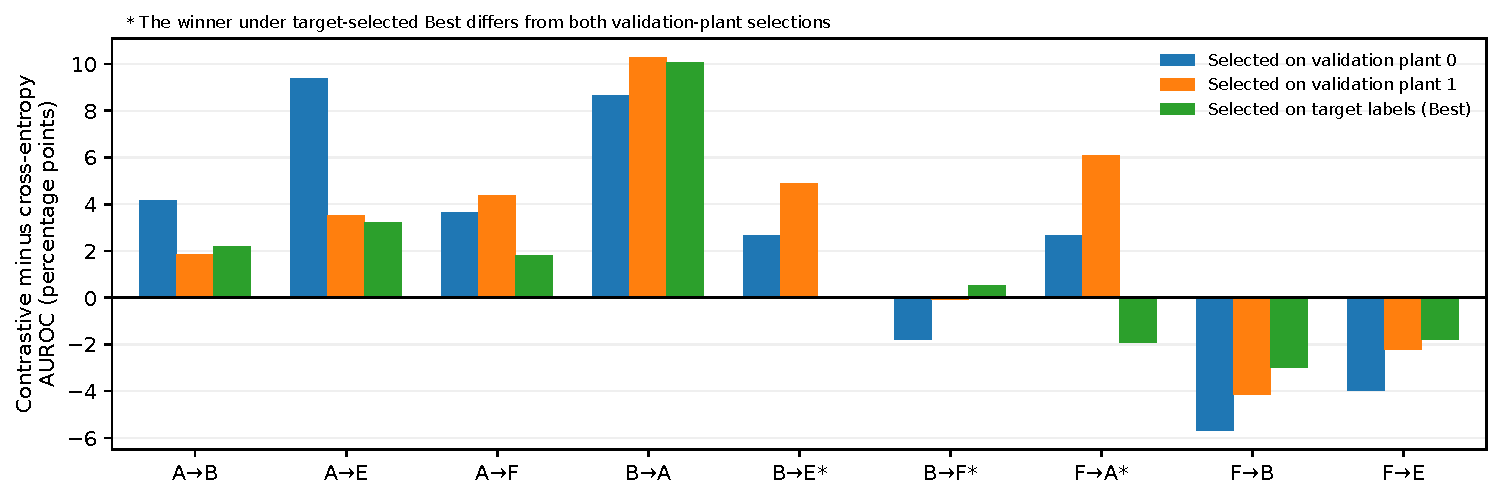
\includegraphics[width=\linewidth]{figures/figure_bommes_condition.pdf}
\caption{Difference in printed AUROC between contrastive and cross-entropy classifiers for nine source--target PV plant tasks under three different published checkpoint-selection conditions. Positive values favor contrastive; negative values favor cross-entropy. Asterisks identify strict direction changes versus \emph{both} validation-plant conditions. The original authors report these outcomes; our contribution is the source-bound, transparent separation by checkpoint rule, not a new PV experiment.}
\label{fig:selection}
\end{figure}

The largest reported target-best minus validation-plant differences are \textbf{11.71} points for contrastive and \textbf{19.73} points for cross-entropy, both on F$\rightarrow$A relative to validation condition 1 (73.29 versus 61.58 and 75.22 versus 55.49, respectively). These values come from simple subtraction of Table~5 entries and do not establish target leakage, incorrect methodology, or an inflation rate. Indeed, the authors explicitly discuss why knowing the target's labels is unavailable in deployment and investigate validation on another plant. A careful review should use this source as a \emph{positive disclosure case}: when selection conventions are transparent, the scope of the reported score is identifiable. A distinct interval check that permits each two-decimal reported AUROC cell to vary by up to 0.005 percentage points (and a pairwise method difference by 0.010) retains all three printed ordering reversals. This is \emph{display-rounding robustness only}, not a bootstrap, uncertainty of the underlying three runs, or statistical significance.

\subsection{Image grouping, physical grouping and task support are distinct}
A second original-source case reports 1,560 thermal images and a 70/15/15 \emph{module-wise} partition for a six-class classification exercise; the same paper describes a separate 124-image hotspot-segmentation reference subset \cite{decarlo2026}. Its reported Random Forest accuracy of 97.6\% is a classification result, not a segmentation result or a newly tested camera/site performance guarantee. The published grouping policy is informative, but an independent complete mapping of images to modules and new facilities was not replayed here.

Bayat Toksoz et al. report five-fold group-aware EL classification across 17,377 image observations and 17,324 available source-group identifiers \cite{bayat2026}. The arithmetic difference, 53, does \emph{not} identify 53 duplicates, 17,324 independent modules, or physical-parent disjointness. The same publication reports macro-F1 of 79.92\% for one parameter-efficient configuration and 78.26\% for full fine-tuning within its defined grouped-CV setting; the two training-memory figures 1,727 MB and 2,478 MB were obtained with different batch sizes, so their difference is not an isolated quantization effect. These are useful reproducible source observations and specifically bounded comparisons.

A separately tracked contemporary paper reports 0.8876 internal AUROC for a PVEL-AD held-out test cohort, followed by a transferred calibrated anomaly score saturating to one on all 2,624 ELPV images; its primary endpoint-label subset has 2,223 cases, for which the author reports AUROC 0.5000 \cite{calisan2026}. This directly illustrates why a held-out score on one dataset cannot be silently presented as an externally valid score on a second dataset. The source itself distinguishes its subsequent uncalibrated post-hoc diagnostics from the original zero-shot calibrated transfer. The paper was discovered after the database-search freeze although the publisher dates its publication to 21 October 2026, ten days before that freeze. An independent literal DOI and title check of the original 5,440 provisional identities found neither. This is a bounded \emph{search-frame coverage observation}, not proof that the October search strategy failed or that providers indexed the article by the query date. Its results remain contextual only until the search/additional-source and eligibility record are reconciled.

\begin{table}[ht]
\centering\small
\caption{Illustrative source-to-claim distinctions. Entries are individual experimental contexts, not a random or complete study sample.}
\begin{tabularx}{\linewidth}{@{}p{2cm}p{2.3cm}X X@{}}
\toprule Source & Reported experiment & Defensible source statement & Stronger claim remaining unresolved \\
\midrule Bommes et al. \cite{bommes2022} & Cross-plant IR anomaly classification; two checkpoint regimes & Printed AUROC depends on checkpoint choice; author reports grouped modules and cross-plant tasks & Fully untouched target-label selection for target-best; independent raw parent and checkpoint replay \\
De Carlo et al. \cite{decarlo2026} & Thermal fault classification and separate mask subset & Authors describe module-wise splitting; distinct task denominators & New camera/site transfer; independently verified image--module map \\
Bayat Toksoz et al. \cite{bayat2026} & Five-fold group-aware EL classification & Author-reported fold identifiers and metric family & Complete physical module ancestry and external-site evaluation \\
Calisan \cite{calisan2026} & Internal PVEL-AD test; ELPV score transport & Source reports a failed calibrated transfer on a different EL family & An externally verified new-site failure rate, extrapolated population prevalence \\
\bottomrule
\end{tabularx}
\end{table}

\subsection{Source-version alignment is a separate identifiability gate}
An illustrative 2026 preprint's public abstract describes a four-class, two-modality SolarFCD dataset comprising 4,435 images \cite{solarfcd2026}. Its linked official code repository README, as inspected at its publicly available version, describes 3,742 images and a train/validation/test layout of 3,030/337/375, which correctly sums to 3,742 \cite{solarfcdrepo}. The two public descriptions differ by 693 images. Without the precise full paper protocol, archival dataset version and image-ID correspondence, this is a \emph{source-release alignment question}, not a demonstration of a data error, leakage, or invalid reported model accuracy. The example also shows why an author's current README should not be treated as proof of the images or source preprocessing used in a reported earlier experiment. SolarFCD is a contextual repository case; no new frozen-source inclusion is asserted.

\subsection{Source-key independence changes the admissible testing population}
Original Sandia metadata yield 269 single-observation, 160 two-observation and nine three-observation module IDs, or 169 repeatedly measured modules and 347/616 acquisition rows belonging to them. Under the 100 actual row-wise random partitions, a mean 55.17 distinct \texttt{Mod\_ID}s occur in both training and test (range 38--70); an average 45.3821\% of held-out acquisition rows have a module identifier present in training. All 100 whole-module partitions have \emph{zero} common \texttt{Mod\_ID}s. Conditional on the observed multiplicity vector, the exact row-random expectation is 55.5425 shared modules. These are 100 design variations on \emph{one public metadata archive}, not 100 new field cohorts or evidence that a particular published model used an invalid split. In these two designs the test support is different: a random-row holdout is a mixture of previously observed and unseen module identities, whereas whole-module grouping excludes every training module from its test set. Consequently the contrast describes two evaluation populations, rather than isolating the causal effect of removing parent overlap.

\begin{figure}[ht]\centering
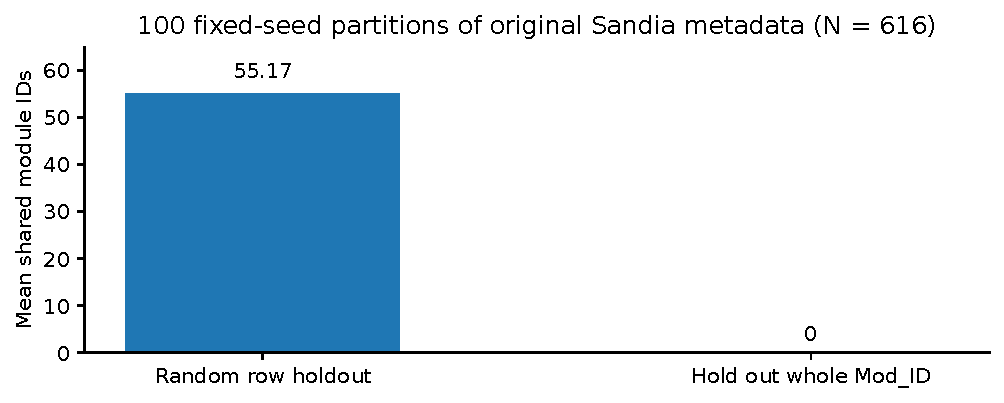
\includegraphics[width=0.84\linewidth]{figures/figure_sandia_module_overlap.pdf}
\caption{Executed original-metadata support diagnostic: mean number of Sandia source-module identifiers in both training and test across 100 fixed-seed partitions (616 acquisition rows). Grouped zero overlap is guaranteed by the partition rule and independently checked. This is not observed EL defect detection or model-score leakage.}
\label{fig:sandia}
\end{figure}

The source has 613 distinct \texttt{IVPath} values but 616 nonidentical metadata rows. Exactly three IV paths are reused, each linked to distinct EL acquisition entries; this is a \emph{numeric catalog count bridge}, not proof of the publisher's historical counting convention. The 600 rows carrying both high- and low-current EL links span 435 module IDs and 599 unique IV paths. Among them, 479/600 have EL and IV acquisition dates within $\pm 7$ days, while 121 are farther apart. Source paths are not independently verified image bytes. Neither source-row deduplication nor EL--IV contemporaneity is an automatic modeling assumption.

\subsection{A non-imaging predictive negative control does not show material inflation}
For the 598-row fixed electrical-ratio cohort, mean source-module overlap under row-wise selection is 56.17, versus zero under whole-module selection. The fixed, non-ID metadata Ridge achieves mean MAE 0.8650 ratio percentage points under row partitions and 0.8790 under grouped partitions (difference $-0.0140$ points). Under row-wise splitting, 47.5083\% of held-out records have a \texttt{Mod\_ID} also present in training on average; this identity-overlap fraction is not a prediction-error effect size. A constant-nameplate model yields 1.9735 and 1.9656 points, respectively. Row-wise Ridge has lower MAE in 57/100 repeated seeds but the opposite holds in 43; signed row-minus-group differences range from $-0.3041$ to $+0.2723$ points. The seeds reuse the same dataset, test populations differ and no inferential $p$-value or causal optimism is estimated. The result matters precisely because it \emph{does not} demonstrate a universal score penalty: source-overlap and score inflation are distinct empirical questions. Methods on dependence-structured data and cross-validation variability explain why that distinction is material \cite{roberts2017,varoquaux2018}.

\begin{table}[ht]\centering\small
\caption{Executed Sandia source-key and non-imaging outcome controls. Different analytic cohorts and endpoints are not pooled.}
\begin{tabularx}{\linewidth}{@{}p{3.2cm}XX@{}}\toprule
Diagnostic & Random rows (100 seeds) & Whole-module grouping (100 seeds) \\ \midrule
Original 616-row source membership & 55.17 shared \texttt{Mod\_ID}s; range 38--70 & Zero shared \texttt{Mod\_ID}s \\
Fixed 598-row nonimage Ridge cohort & 56.17 shared \texttt{Mod\_ID}s & Zero shared \texttt{Mod\_ID}s \\
Measured electrical $P_{\rm mp}$/nameplate MAE & 0.8650 ratio pp & 0.8790 ratio pp \\
Constant-nameplate MAE & 1.9735 ratio pp & 1.9656 ratio pp \\
\bottomrule\end{tabularx}
\end{table}

\subsection{A future calendar test is neither an unseen-module test nor guaranteed EL support}
An independently source-hash-verified 598-row Sandia subset spans 420 source-module identifiers and 33 distinct IV acquisition dates. A predeclared, intact-calendar-date test block beginning 9 February 2021 has 139 later IV observations; 459 observations are earlier. The later test shares \emph{56} source \texttt{Mod\_ID}s with earlier training, and 56 test records have a source-module identifier already present in the earlier records. Removing the 59 earlier rows associated with these test modules yields 400 training rows that are both earlier in time and \texttt{Mod\_ID}-disjoint from the unchanged 139-row future test. This changes the eligible training population; it does not create a randomized leakage-removal experiment.

The pre-locked R52 non-imaging Ridge fitted on all 459 earlier source records has future-test MAE \textbf{1.3691} ratio percentage points and 4.3965 W. Excluding the 59 earlier test-shared records increases the \emph{same 139-row test} MAE to \textbf{1.6411} ratio percentage points and 5.2684 W (difference +0.2720 ratio points). With 100 predeclared size-matched alternatives that each drop 59 other earlier records but retain the future-seen module observations, mean MAE is 1.4019 ratio points; all 100 are below 1.6411. This control shows that training-count loss alone is not a sufficient description of the observed numerical contrast, but \emph{does not} isolate a causal effect of overlap: training composition and source-module selection remain confounded. A separate R52 row-versus-grouped diagnostic obtained much closer errors on \emph{different} held-out units; these are different estimands and are not contradictory.

\begin{table}[ht]\centering\small
\caption{Same-future-test source support: original Sandia metadata, non-imaging IV-power-ratio Ridge, not EL-defect detection.}
\begin{tabularx}{\linewidth}{@{}p{4.0cm}X X@{}}\toprule
Design / source support & Earlier fitting records & Identical future test (139 rows) \\ \midrule
Complete-date boundary & 459; 56 module IDs shared & 139; 56 previously seen module IDs \\
Conjunctive date + module disjointness & 400; 0 IDs shared & 139; 0 IDs shared with retained train \\
Paired EL paths with same-date channels, within 7 days of IV & 401/459 original earlier & 60/139 later \\
Non-imaging Ridge ratio MAE, all earlier / disjoint earlier & 1.3691 / 1.6411 ratio pp & Both evaluated on the same 139 rows \\
\bottomrule\end{tabularx}
\end{table}

The near-date paired EL-path metadata fraction is 401/459 (87.36\%) in the original earlier cohort but only 60/139 (43.17\%) in the later cohort. These are \emph{recorded links and date fields}, not verified TIFF pixels. They establish a separate, outcome-independent \emph{eligibility-support shift} in any subsequent EL-plus-IV experiment, not a model error for image recognition, chronology-driven degradation, or proof of cross-site transfer.

\subsection{File disjointness is weaker than candidate source-family disjointness}
Pinned public Git trees for Pratt et al.'s EL segmentation repository \cite{pratt2023} show zero \emph{identical} train/test crop filenames in each of three dated releases. Yet the restricted, explicitly labeled filename-prefix parser finds 22, 33 and 34 cross-partition candidate families, respectively (in 2021-11, 2022-07 and 2022-10 versions). The corresponding test images with a parsed family also in training are 24/50, 35/66 and 36/72 total test entries. Unparsed image families remain unknown. In the 2021 release, all 1,434 augmented training filenames map exactly to 478 original training crop filenames, three derivatives per original, demonstrating a documented training-only augmentation pattern. Original-author documentary evidence now qualifies the filename interpretation: Pratt's 2024 thesis associates the 2021-11-04 public dataset release with the 2023 benchmark paper family and explicitly describes CFVS-00035-r8-c4 as a crop from source \emph{module 00035}, row 8, column 4 \cite{prattthesis2024}. The 2021 Git tree and thesis agree on 478 original training, 54 validation and 50 test images (582 total), with 1912 training images including training-only augmentation. The separate journal report's 593-image statement remains an 11-image reconciliation HOLD. The author describes a defect-enriched, deliberately selected 50-image test set, not a representative new-deployment cohort. A fresh source-specific recount yields ARTS/CFVS/CSIR matched train--test keys of 8/8/6 in 2021, 10/12/11 in 2022-07 and 10/11/13 in 2022-10. These observations strengthen one original-source name-semantic interpretation but do not certify unique physical module serials for all prefixes, exact journal-model training assets, image-pixel duplication or a change in published mIoU.

\begin{table}[ht]\centering\small
\caption{Source-to-claim changes in executed examples. None certifies a paper-specific leaked model.}
\begin{tabularx}{\linewidth}{@{}p{2.0cm}X X@{}}\toprule
Case & Verified observation & Maximum defensible conclusion \\ \midrule
Bommes 2022 & Three of nine author-reported AUROC task orderings depend on checkpoint choice & The selection rule qualifies the reported comparison, not a causal leakage effect \\
Sandia 2025 & 55.17 shared modules with random rows versus zero grouped & The held-out population changes at a declared physical \texttt{Mod\_ID} level \\
Sandia R52 control & Non-imaging MAE 0.8650 versus 0.8790 ratio pp & Overlap does not by itself prove optimistic predictive error \\
Pratt repository & 0 duplicate filenames, 22/33/34 matched candidate-name families & No physical-parent or paper-model inference without an author crosswalk \\
\bottomrule\end{tabularx}
\end{table}

\subsection{Printed dataset and metric denominators are independent source gates}
Two further original-document checks show why printed counts and measure definitions must remain attached to individual results. El-Rashidy's EL classifier paper describes a benchmark of 2,624 cell images in its Introduction but refers to 2,426 in the Experimental Results section; the latter describes 44 source panels and fivefold cross-validation \cite{elrashidy2022}. The visible difference is 198 images, yet neither an image-exclusion crosswalk nor a fold-to-physical-panel manifest was obtained. This textual discrepancy is \emph{not} proof of an incorrect result or a contaminated image split.

In a different thermographic segmentation paper, Oulefki et al.\ print the Jaccard/IoU formula as $\mathrm{TP}/(\mathrm{TP}+\mathrm{FN})$ in Table 4, identically to the table's recall formula \cite{oulefki2024}. The conventional binary-mask IoU is $\mathrm{TP}/(\mathrm{TP}+\mathrm{FP}+\mathrm{FN})$. For a \emph{synthetic} example with $\mathrm{TP}=20$, $\mathrm{FP}=10$, and $\mathrm{FN}=5$, the former evaluates to $0.800$ and the latter to $0.571$. The discrepancy concerns the \emph{printed formula}, not independently inspected implementation: code and true masks were not replayed, and the original paper's Table 5 scores are neither recalculated nor invalidated here.

\begin{table}[t]
\centering\small
\caption{Two original-document reporting observations and the stronger result claims still unresolved. Neither observation proves defective study results or actual data leakage.}
\begin{tabularx}{\linewidth}{@{}p{0.24\linewidth}XX@{}}
\toprule
Report & Original source-visible statement & Claim not established \\
\midrule
El-Rashidy (2022) & 2,624 source images in Introduction; 2,426 in Experiments, with 44 panels & Actual image inclusion rule, source-to-fold physical parent map \\
Oulefki et al.\ (2024) & IoU printed as TP/(TP+FN), identical to recall & Whether the printed expression was used by the source code; corrected test-mask metrics \\
\bottomrule
\end{tabularx}
\end{table}

\subsection{A reusable claim-support object, not a quality score}
The accompanying JSON Schema and executable examples require the source and experiment identifiers, image modality, target task, evaluation unit, split-disjointness unit, source tier, physical-parent crosswalk status, target-label selection exposure, metric unit/support and requested claim. A rule refuses to upgrade a paper's author-described module-wise split to a \raw{} physical-parent certificate unless a raw parent manifest is actually replayed and the claimed partition has verified zero overlap. A separate rule blocks an ``untouched target-model selection'' assertion when target labels are recorded as selecting the Best checkpoint. These are transparent reporting rules and test fixtures, not empirical estimates of publication validity or a novel prediction model. No illustrative empirical case is given a raw-replayed physical-disjointness certificate in this draft.

\section{Scientific interpretation and limitations}
The central observation is a distinction between \emph{observable reporting support} and \emph{true but unavailable experimental conditions}. Physical independence is conditional on a parent relation (image, original capture, cell, module, batch, flight, date or plant) and on an explicit boundary between data used in fitting, tuning and outcome estimation. An author may correctly use a grouped split without publishing every manifest needed for independent verification. Conversely, the presence of multiple plants or many augmented images cannot by itself prove an untouched test cohort. The intent of the proposed record is to make these statements precise, not to discredit high-performing models.

This manuscript is not yet a completed systematic review. The initial W4 source screen remains incomplete; later full-text eligibility, source-depth evidence reconciliation, bibliographic identity arbitration and formal PRISMA/PRISMA-S reporting are unclosed. The early 599-group retrieval priority is \emph{not} a representative sample from which to estimate the prevalence of leakage or validation practice. AI-assisted screening is reported as a single AI-assisted source-screen process; no second independent human reviewer or kappa is invented. Neither the currently available source texts nor the hash-matched bibliographic files demonstrate every trained checkpoint's physical disjointness. The published result contexts are purposively selected; 54 Bommes cells belong to \emph{one} source paper and cannot be treated as 54 independent studies. The new Sandia diagnostics concern one original metadata archive and an electrical endpoint, not defect-classification accuracy. The future-cohort comparison keeps the evaluation observations fixed but alters training size and composition; the equal-size negative control is not a randomized removal of physical overlap. The original Pratt thesis supplies an author-described module-number pattern for one file family without an independently traced per-file physical serial crosswalk. The 100 randomized seeds and the three versioned Git trees are correlated design/release checks, not independent study replicates. Statistical significance, causal bias adjustment, pooled accuracy and site-transfer rates are not estimated.

The novelty claim has a further constraint: prior reviews already tabulate original and augmented PV image counts, split allocations, datasets and model results; several 2026 reviews also identify dataset heterogeneity and evaluation-metric comparability problems \cite{ali2026,meena2026,ieee2026,rahman2026,pillai2027}. Prior-art comparison here is verified at heterogeneous source tiers (some publisher abstracts, one complete open full text) and is not an exhaustive claim that no predecessor has ever proposed a structured validation-audit checklist. A stronger final submission would systematically distinguish which competing works actually execute source-version/physical-parent/checkpoint/result-level checks, rather than saying only that they ``mention'' datasets.

\section{Conclusion and next evidence gate}
A citable methodological contribution is possible if the final paper demonstrates a consistent, reproducible mapping from published PV defect-image results to the specific experiment and statistical unit their evidence supports. The present bounded reproduction shows why checkpoint selection matters: in a transparent nine-task cross-plant study, the reported model ordering can depend on whether labels from another PV plant or the target plant determine the reported checkpoint. Complementary examples show that author-reported module-grouping, source-grouped folds and calibration transfer each address a different evidentiary question. The next necessary work is to complete the outstanding source and full-text screening and close the final PRISMA-S and identity gates while preserving exact source provenance and a publicly releasable version of the audit scripts, and original EL pixels where a predictive image-based comparison is justified. The new date-block and module-identity joint audit shows why a future PV evaluation needs both a declared target clock and a physical-parent support rule; its measured non-imaging error contrast must not be extrapolated to fault-classification performance. Strong claims about actual leakage, external generalization prevalence, or a pooled model leaderboard are not warranted by the present evidence.

\section*{AI assistance and author verification status}
AI assistance supported literature triage, source-ledger construction, drafting and code scaffolding. Reported computations are checked against archived inputs and deterministic scripts; a second independent human eligibility screen has not occurred. The authors must review scientific decisions, approved source redistribution and journal-required AI disclosures before submission. This text does not assert that author-side independent verification or final approval has already occurred.

\section*{Data, code and integrity}
The executable source, reproducible derived analyses, experiment-indexed claim schema and accompanying development PDFs are now publicly accessible at \href{https://github.com/shaikhamalkawi-ux/pv-imaging-validation-audit}{the public Project~99pv repository}. The source-verified R54 code snapshot is pinned to commit \href{https://github.com/shaikhamalkawi-ux/pv-imaging-validation-audit/commit/b0bf66f9670000297986569dab6de85d55bec822}{\texttt{b0bf66f96700}}; the public GitHub Actions workflow passed its bounded offline source-table, manifest-name parser and mathematical self-checks. Those checks do \emph{not} rerun Sandia predictions without the separately obtained original data. The archival original metadata SHA, original-source DOI and published Git-tree identifiers are recorded in the repository. Neither Sandia EL/IV original archives nor private institutional bibliographic exports or third-party publisher PDFs are redistributed. New R57 code and aggregate-only source evidence for the date-blocked Sandia control, plus author-thesis/stratified public-tree lineage data, are published separately; the live public test workflow verifies only bounded source-independent calculations unless the original Sandia CSV is obtained and hashed. R53 true EL-pixel evaluation remains a frozen prospective protocol, not a result. Public availability does not itself grant reuse rights; author-level licensing, final metadata, adjudicated PRISMA and eligibility remain pending. \cite{wilkinson2016}

\begin{thebibliography}{99}\small\setlength{\itemsep}{1pt}
\bibitem{prisma} Page MJ et al. The PRISMA 2020 statement: an updated guideline for reporting systematic reviews. \emph{BMJ}. 2021;372:n71. doi:10.1136/bmj.n71.
\bibitem{prismas} Rethlefsen ML et al. PRISMA-S: an extension to the PRISMA Statement for Reporting Literature Searches in Systematic Reviews. \emph{Systematic Reviews}. 2021;10:39. doi:10.1186/s13643-020-01542-z.
\bibitem{ali2026} Ali MU, Zafar A, Kim KS. Imaging based fault diagnosis of photovoltaic modules: a systematic review. \emph{Solar Energy}. 2026;314:114679. doi:10.1016/j.solener.2026.114679.
\bibitem{meena2026} Meena S, Gawre SK. Encapsulating intelligent fault analysis in solar PV arrays: From conventional to AI-driven techniques. \emph{Sustainable Energy Technologies and Assessments}. 2026;91:105041. doi:10.1016/j.seta.2026.105041.
\bibitem{ieee2026} Common Failures in Photovoltaic Systems and Their Diagnostic Methods With Applications of Artificial Intelligence Techniques: A Review. \emph{IEEE Access}. 2026;14:159245--159290. doi:10.1109/ACCESS.2026.3742570. [Author metadata to verify before submission.]
\bibitem{rahman2026} Rahman MM, Srivastava AK. Detection, classification, and localization of faults and failures in photovoltaic arrays: a review, comparative analysis, and path forward. \emph{Discover Energy}. 2026;6:26. doi:10.1007/s43937-026-00136-5.
\bibitem{pillai2027} Pillai DS et al. Benchmarking imaging-based inspection techniques for PV systems. \emph{Renewable and Sustainable Energy Reviews}. Publisher/indexer listed for 2027;244:117457. doi:10.1016/j.rser.2026.117457. [Online/final issue status to re-verify.]
\bibitem{li2021} Li B, Delpha C, Diallo D, Migan-Dubois A. Application of Artificial Neural Networks to Photovoltaic Fault Detection and Diagnosis: A Review. \emph{Renewable and Sustainable Energy Reviews}. 2021;138:110512. doi:10.1016/j.rser.2020.110512.
\bibitem{wangxing2026} Wang Y, Xing Y. Artificial Intelligence-Based Defect Prediction in Photovoltaic Panels Coupling with Nondestructive Detection Techniques: A Comprehensive Review. \emph{Energy Technology}. 2026;14(1):e202502065. Online December 2025. doi:10.1002/ente.202502065.
\bibitem{nasri2026} Nasri I, Mansouri M, Trabelsi M, Khriji L, Skorek AW. A Review on Multimodal-Based Fault Detection and Diagnosis in Photovoltaic Systems: Fusion and Attention Mechanisms. \emph{IEEE Access}. 2026;14:44382--44402. doi:10.1109/ACCESS.2026.3675686.
\bibitem{lu2026} Lu W-Q, Delpha C, Diallo D, Migan-Dubois A. A comprehensive review of fusion-based methods applied to photovoltaic fault diagnosis. \emph{Solar Energy}. 2026;309:114457. doi:10.1016/j.solener.2026.114457.
\bibitem{elrashidy2022} El-Rashidy MA. An efficient and portable solar cell defect detection system. \emph{Neural Computing and Applications}. 2022;34:18497--18509. doi:10.1007/s00521-022-07464-2.
\bibitem{oulefki2024} Oulefki A, Himeur Y, Trongtirakul T, et al. Detection and analysis of deteriorated areas in solar PV modules using unsupervised sensing algorithms and 3D augmented reality. \emph{Heliyon}. 2024;10(6):e27973. doi:10.1016/j.heliyon.2024.e27973.
\bibitem{bommes2022} Bommes L, Hoffmann M, Buerhop-Lutz C, Pickel T, Hauch J, Brabec C, Maier A, Peters IM. Anomaly detection in IR images of PV modules using supervised contrastive learning. \emph{Progress in Photovoltaics}. 2022;30:597--614. doi:10.1002/pip.3518.
\bibitem{decarlo2026} De Carlo D, Calcagno S, Angiulli G. An Intelligent Thermographic Framework for Automated Diagnosis and Health Monitoring of Photovoltaic Modules. \emph{Applied Sciences}. 2026;16:9018. doi:10.3390/app16189018.
\bibitem{bayat2026} Bayat Toksoz S, Isik G, Sahin G, Akin E. Parameter-Efficient Fine-Tuning for Photovoltaic Cell Defect Classification: A Systematic Comparison of LoRA, QLoRA, and Full Fine-Tuning on ConvNeXt-Tiny. \emph{Sensors}. 2026;26:3659. doi:10.3390/s26123659.
\bibitem{solarfcd2026} Ijaz M, Khan SUR, Rehman AU, Zaib A, Vollmer S, Dengel A, Asim MN. SolarFCD: A Large-Scale Dataset and Benchmark for Solar Fault Classification in Photovoltaic Systems. arXiv:2604.23662, submitted 26 April 2026. \url{https://arxiv.org/abs/2604.23662}.
\bibitem{solarfcdrepo} VS-EYE. SolarFCD public code repository and dataset description. \url{https://github.com/VS-EYE/SolarFCD}. Version and image-parent snapshot correspondence pending; accessed 7 November 2026.
\bibitem{calisan2026} \c{C}al{\i}\c{s}an M. Structure-Aware Photovoltaic EL Anomaly Detection with Frozen DINOv2. \emph{Sustainability}. 2026;18:10677. doi:10.3390/su182010677. Published 21 October 2026.
\bibitem{sandia2025} Braid J, Byford B, Theristis M, Robinson C, Snyder W, Santistevan K, Jost N, King B. Photovoltaic Module Current-Voltage and Electroluminescence Image Data (PV-IV-EL). Sandia National Laboratories / OEDI public dataset, 2025. Dataset doi:10.11578/3818365.
\bibitem{byford2025} Byford BK, Boucheron LE, King BH, Braid J. Advanced Photovoltaic Module Characterization: Using Image Transformers for Current--Voltage Curve Prediction From Electroluminescence Images. \emph{IEEE Journal of Photovoltaics}. 2025;15(4):557--565. doi:10.1109/JPHOTOV.2025.3562931.
\bibitem{prattthesis2024} Pratt LE. \emph{Deep Learning Models for Defect Detection in Electroluminescence Images of Solar PV Modules}. PhD thesis, University of the Witwatersrand, 2024. \url{https://hdl.handle.net/10539/42163}.
\bibitem{pratt2023} Pratt L, Mattheus J, Klein R. A benchmark dataset for defect detection and classification in electroluminescence images of PV modules using semantic segmentation. \emph{Systems and Soft Computing}. 2023;5:200048. doi:10.1016/j.sasc.2023.200048. Public dataset project \url{https://github.com/TheMakiran/BenchmarkELimages} (tree SHA and publication-version bridge recorded separately).
\bibitem{roberts2017} Roberts DR et al. Cross-validation strategies for data with temporal, spatial, hierarchical, or phylogenetic structure. \emph{Ecography}. 2017;40:913--929. doi:10.1111/ecog.02881.
\bibitem{varoquaux2018} Varoquaux G. Cross-validation failure: Small sample sizes lead to large error bars. \emph{NeuroImage}. 2018;180:68--77. doi:10.1016/j.neuroimage.2017.06.061.
\bibitem{kapoor2023} Kapoor S, Narayanan A. Leakage and the reproducibility crisis in machine-learning-based science. \emph{Patterns}. 2023;4:100804. doi:10.1016/j.patter.2023.100804.
\bibitem{wilkinson2016} Wilkinson MD et al. The FAIR Guiding Principles for scientific data management and stewardship. \emph{Scientific Data}. 2016;3:160018. doi:10.1038/sdata.2016.18.
\end{thebibliography}
\end{document}
